\documentclass[12pt, twoside]{article}
\usepackage[letterpaper, margin=1in, headsep=0.5in]{geometry}
\usepackage[english]{babel}
\usepackage[utf8]{inputenc}
\usepackage{amsmath}
\usepackage{amsfonts}
\usepackage{amssymb}
\usepackage{tikz}
\usetikzlibrary{quotes, angles}
\usepackage{graphicx}
\usepackage{enumitem}
\usepackage{multicol}

\newif\ifmeta
\metatrue %print standards and topics tags

\title{Regents Geometry}
\author{Chris Huson}
\date{September 2020}

\usepackage{fancyhdr}
\pagestyle{fancy}
\fancyhf{}
\renewcommand{\headrulewidth}{0pt} % disable the underline of the header
\raggedbottom


\fancyhead[LE]{\thepage}
\fancyhead[RO]{\thepage \\ Name: \hspace{4cm} \,\\}
\fancyhead[LO]{BECA / Dr. Huson / Geometry 01-Intro\\* pset ID: 6}

\begin{document}

\subsubsection*{1-4HW-Intro}
\begin{enumerate}
\item The points where a line segment begins and ends are the $\rule{4cm}{0.15mm}$. \smallskip
\item A(n) $\rule{4cm}{0.15mm}$ is a portion of a line that includes two points and all of the collinear points between the two points.\smallskip
\item A(n) $\rule{4cm}{0.15mm}$ is a portion of a line that begins with a single point and extends infinitely in one direction.
\item Points that are all located on the same line are $\rule{4cm}{0.15mm}$.\bigskip
\item Two or more line segments of equal measure are $\rule{4cm}{0.15mm}$.\bigskip
\item A flat surface is a(n) $\rule{4cm}{0.15mm}$. \bigskip
\item A(n) $\rule{4cm}{0.15mm}$ is a straight continuous arrangement of an infinite number of points.

\item Use symbols to write the name of each geometric figure.
  \begin{enumerate}
  \item %Ray DE
    \begin{tikzpicture}
      \draw [->, thick] (0,0)--(3,1.5);
      \draw [fill] (0,0) circle [radius=0.05] node[below]{$D$};
      \draw [fill] (2,1) circle [radius=0.05] node[below]{$E$};
    \end{tikzpicture} \bigskip
  \item \hspace{1cm}%Line AB
    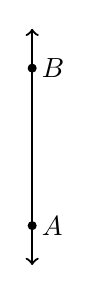
\begin{tikzpicture}
      \draw [<->, thick] (1,0)--(1,3);
      \draw [fill] (1,0.5) circle [radius=0.05] node[right]{$A$};
      \draw [fill] (1,2.5) circle [radius=0.05] node[right]{$B$};
    \end{tikzpicture} \bigskip
    \item %Line segment XY
      \begin{tikzpicture}
        \draw [-, thick] (1,0)--(0,2);
        \draw [fill] (1,0) circle [radius=0.05] node[below]{$X$};
        \draw [fill] (0,2) circle [radius=0.05] node[left]{$Y$};
      \end{tikzpicture}
  \end{enumerate}

\newpage
\subsubsection*{Do Now 1.4: Notation and terminology} % DONE
\item I have a compass, ruler, protractor, notebook, and folder (circle one). Yes \qquad No

\item Use each term according to its geometric meaning: ``sketch", ``draw", ``construct".
    \begin{enumerate}
      \item $\rule{4cm}{0.15mm}$ is to make a freehand diagram showing important features. \smallskip
      \item $\rule{4cm}{0.15mm}$ is to depict with accurate measures using ruler, protractor, and compass. \smallskip
      \item $\rule{4cm}{0.15mm}$ is a formal, logical process to create geometric figures using only a straightedge and compass.
    \end{enumerate} \smallskip

\item Two or more line segments of equal measure are $\rule{4cm}{0.15mm}$.
    \bigskip
\item Given $\overline{ABC}$, $AB=10$, and $BC=4$.
  \begin{enumerate}
    \item Find ${AC}$.\\[0.75cm]
      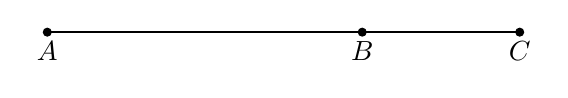
\begin{tikzpicture}
        \draw [-, thick] (1,0)--(7,0);
        \draw [fill] (1,0) circle [radius=0.05] node[below]{$A$};
        \draw [fill] (5,0) circle [radius=0.05] node[below]{$B$};
        \draw [fill] (7,0) circle [radius=0.05] node[below]{$C$};
      \end{tikzpicture} \smallskip
    \item The postulate used in this problem is the \rule{6cm}{0.15mm}.
  \end{enumerate}
  \smallskip

\item Given $\triangle ABC$ with $\overline{AC} \cong \overline{BC}$. On the diagram mark the congruent line segments with tick marks.
  \begin{center}
  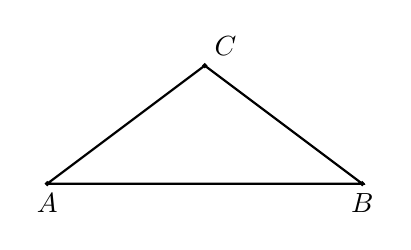
\begin{tikzpicture}[scale=0.5]
    \draw [thick](0,0)--(8,0)--(4,3)--(0,0);
    \draw [fill] (0,0) circle [radius=0.05] node[below]{$A$};
    \draw [fill] (8,0) circle [radius=0.05] node[below]{$B$};
    \draw [fill] (4,3) circle [radius=0.05] node[above right]{$C$};
  \end{tikzpicture}
  \end{center}

\item Given line segment $\overline{AB}$ with midpoint $M$, that is, $\overline{AM} \cong \overline{BM}$. $AM=2$ cm. Find the length of $\overline{AB}$.\\[0.75cm]
  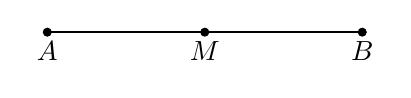
\begin{tikzpicture}
    \draw [-, thick] (1,0)--(5,0);
    \draw [fill] (1,0) circle [radius=0.05] node[below]{$A$};
    \draw [fill] (5,0) circle [radius=0.05] node[below]{$B$};
    \draw [fill] (3,0) circle [radius=0.05] node[below]{$M$};
  \end{tikzpicture}
  \vspace{1cm}

\item Points that are all located on the same line are $\rule{4cm}{0.15mm}$.
\item Find the value of $|8.5-3|$.

\newpage
\item Given the points $X$ and $Y$, draw $\overrightarrow{YX}$.\\
  \vspace{1cm}
  \begin{center}
    \begin{tikzpicture}
    \draw [fill] (0,2) circle [radius=0.05] node[below]{$X$};
    \draw [fill] (5,0) circle [radius=0.05] node[below]{$Y$};
  \end{tikzpicture}
  \end{center}
  %\vspace{2cm}

\item Given $\triangle ABC$ write down two congruent line segments using proper notation.\\
  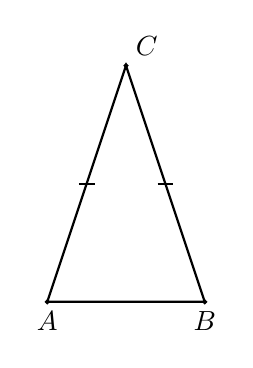
\begin{tikzpicture}[scale=0.5]
    \draw [thick](0,0)--(4,0)--(2,6)--(0,0);
    \draw [fill] (0,0) circle [radius=0.05] node[below]{$A$};
    \draw [fill] (4,0) circle [radius=0.05] node[below]{$B$};
    \draw [fill] (2,6) circle [radius=0.05] node[above right]{$C$};
    \draw [thick] (0.8,3)--(1.2,3); %tick mark
    \draw [thick] (2.8,3)--(3.2,3); %tick mark
  \end{tikzpicture}

\item Given $\overrightarrow{DE}$, construct circle $E$ with radius $DE$.
  \vspace{4cm}
  \begin{center}
  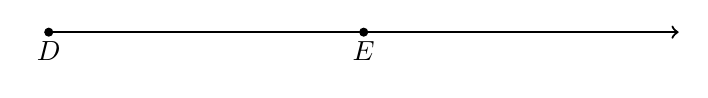
\begin{tikzpicture}
    \draw [->, thick] (0,0)--(8,0);
    \draw [fill] (0,0) circle [radius=0.05] node[below]{$D$};
    \draw [fill] (4,0) circle [radius=0.05] node[below]{$E$};
  \end{tikzpicture}
  \end{center}
  \vspace{4cm}
  Spicy: Complete the construction of an equilateral triangle with one side $\overline{DE}$.

\newpage
\subsubsection*{Homework 1.4: Geometric diagrams}
\item A flat surface is a(n) $\rule{4cm}{0.15mm}$.
\item Use symbols to write the name of the given figure.
  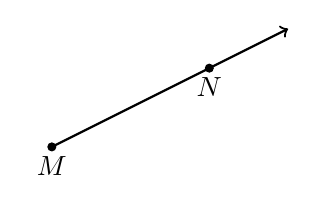
\begin{tikzpicture}
    \draw [->, thick] (0,0)--(3,1.5);
    \draw [fill] (0,0) circle [radius=0.05] node[below]{$M$};
    \draw [fill] (2,1) circle [radius=0.05] node[below]{$N$};
  \end{tikzpicture} \bigskip

\item Given $\overline{ABC}$, $AB=2x+1$, $BC=x-1$, and $AC=9$. Find ${AB}$.\\[0.5in]
    %\vspace{1cm}
    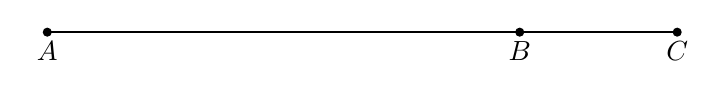
\begin{tikzpicture}
    \draw [-, thick] (-1,0)--(7,0);
    \draw [fill] (-1,0) circle [radius=0.05] node[below]{$A$};
    \draw [fill] (5,0) circle [radius=0.05] node[below]{$B$};
    \draw [fill] (7,0) circle [radius=0.05] node[below]{$C$};
  \end{tikzpicture} \vspace{4cm}

\item Write down the name of two line segments shown in the diagram below using proper geometric notation.
  \begin{center}
  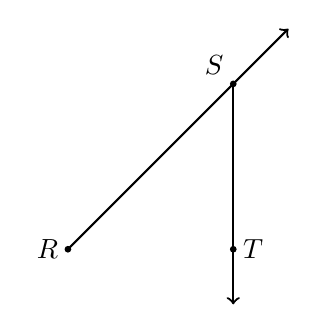
\begin{tikzpicture}[scale=0.7]
    \draw [->, thick] (0,0)--(4,4);
    \draw [->, thick] (3,3)--(3,-1);
    \draw [fill] (0,0) circle [radius=0.05] node[left]{$R$};
    \draw [fill] (3,3) circle [radius=0.05] node[above left]{$S$};
    \draw [fill] (3,0) circle [radius=0.05] node[right]{$T$};
  \end{tikzpicture}
  \end{center}

\item Identify two lines in the given plane.\\[0.25in]
    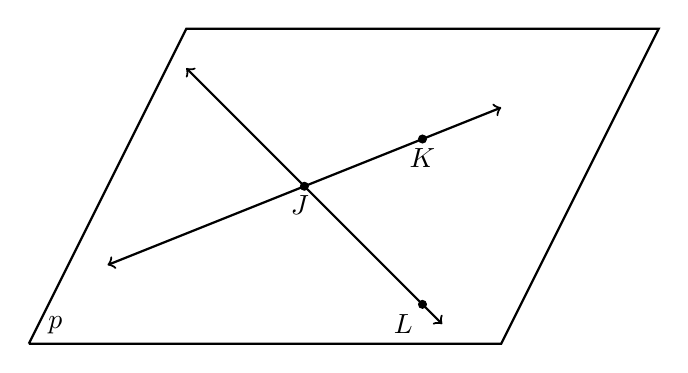
\begin{tikzpicture}
      \draw [thick](0,0) node[above right]{$\ p$} --(6,0)--(8,4)--(2,4)--(0,0);
      \draw [<->, thick] (1,1)--(6,3);
      \draw [fill] (3.5,2) circle [radius=0.05] node[below]{$J \ $};
      \draw [fill] (5,2.6) circle [radius=0.05] node[below]{$K$};
      \draw [<->, thick] (2,3.5)--(5.25,.25);
      \draw [fill] (5,0.5) circle [radius=0.05] node[below left]{$L$};
    \end{tikzpicture} %\vspace{2cm}

\newpage
\item Given $\triangle ABC$ with $\overline{AC} \cong \overline{BC}$. $AC=x+7$ and $BC=2x+1$. Find $AC$.\\[0.5cm]
  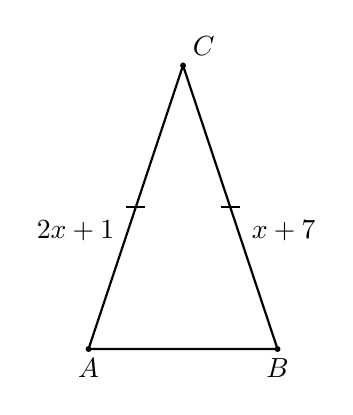
\begin{tikzpicture}[scale=0.6]
    \draw [thick](0,0)--(4,0)--(2,6)--(0,0);
    \draw [fill] (0,0) circle [radius=0.05] node[below]{$A$};
    \draw [fill] (4,0) circle [radius=0.05] node[below]{$B$};
    \draw [fill] (2,6) circle [radius=0.05] node[above right]{$C$};
    \draw [thick] (0.8,3)--(1.2,3); %tick mark
    \draw [thick] (2.8,3)--(3.2,3); %tick mark
    \node [right] at (3.25,2.5){$x+7$};
    \node [left] at (0.75,2.5){$2x+1$};
  \end{tikzpicture}

\item $\rule{4cm}{0.15mm}$ is to make a freehand diagram showing important features. \smallskip

\item Given $A(4,3)$ and $B(6,4)$. What is the slope of $\overleftrightarrow{AB}$? Use the formula $\displaystyle m=\frac{y_2-y_1}{x_2-x_1}$. \vspace{4cm}

\item Points that are all located on the same line are $\rule{4cm}{0.15mm}$.\bigskip

\item Spicy: Given the rectangle $ABCD$ with $\overline{AB} \cong \overline{CD}$ and $\overline{BC} \cong \overline{DA}$. $AB=x+7$ and $\displaystyle CD=\frac{4x+2}{2}$. Find $AB$.\\[0.5cm]
  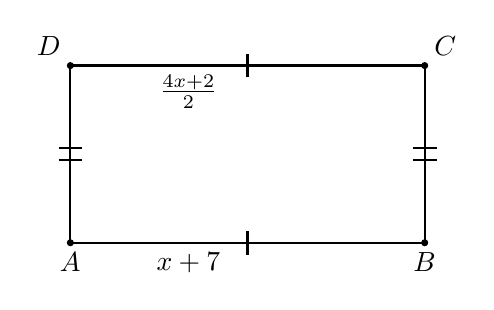
\begin{tikzpicture}[scale=0.75]
    \draw [thick](0,0)--(6,0)--(6,3)--(0,3)--(0,0);
    \draw [fill] (0,0) circle [radius=0.05] node[below]{$A$};
    \draw [fill] (6,0) circle [radius=0.05] node[below]{$B$};
    \draw [fill] (6,3) circle [radius=0.05] node[above right]{$C$};
    \draw [fill] (0,3) circle [radius=0.05] node[above left]{$D$};
    \draw [thick] (3,-0.2)--(3,0.2); %tick mark
    \draw [thick] (3,2.8)--(3,3.2); %tick mark
    \draw [thick] (-0.2,1.4)--(0.2,1.4); %tick mark
    \draw [thick] (-0.2,1.6)--(0.2,1.6); %tick mark
    \draw [thick] (5.8,1.4)--(6.2,1.4); %tick mark
    \draw [thick] (5.8,1.6)--(6.2,1.6); %tick mark
    \node [below] at (2,0){$x+7$};
    \node [below] at (2,3){$\frac{4x+2}{2}$};
  \end{tikzpicture}
  %\vspace{4cm}

\newpage
\subsubsection*{Do Now 1.5: Plane geometry, measure lengths}
\item Accurately measure the length of each side of $\triangle ABC$ in centimeters (cm) to the nearest tenth.
    \bigskip
  \begin{enumerate}
    \item $AB=\rule{2cm}{0.15mm}$ \bigskip
    \item $BC=\rule{2cm}{0.15mm}$ \bigskip
    \item $AC=\rule{2cm}{0.15mm}$
  \end{enumerate}
  \begin{center}
  \begin{tikzpicture}%[scale=0.5]
    \draw [thick](0,0)--(8,1)--(2,4)--(0,0);
    \draw [fill] (0,0) circle [radius=0.05] node[below]{$A$};
    \draw [fill] (8,1) circle [radius=0.05] node[below]{$B$};
    \draw [fill] (2,4) circle [radius=0.05] node[above right]{$C$};
  \end{tikzpicture}
  \end{center}

\item Draw a figure for each description. Draw the line or segment and label all points mentioned in the description.
  \begin{enumerate}
    \item The line segment $XY$ such that the distance between points $X$ and $Y$ is 6 cm. \vspace{2cm}
    \item Points $A$, $D$, and $X$ are collinear such that point $A$ is located halfway between points $D$ and $X$. (hint: mark the congruent segments with tick marks) \vspace{2cm}
    \item Points $A$, $B$, and $C$ are collinear such that point $B$ is between points $A$ and $C$ and the distance between points $A$ and $B$ is twice the distance between points $B$ and $C$. \vspace{2cm}
  \end{enumerate}

\newpage
\subsubsection*{Homework 1.5: Segment addition. Reminder construction project due tomorrow}
\item Given $\overline{ABC}$, $AB=4x-9$, $BC=x+11$, $AC=22$. Find ${AB}$. Show each step:\\[0.5in]
  \begin{center}
    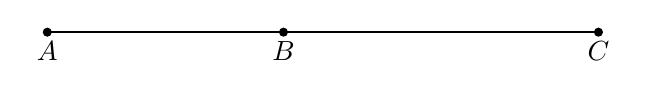
\begin{tikzpicture}
        \draw [-, thick] (0,0)--(7,0);
        \draw [fill] (0,0) circle [radius=0.05] node[below]{$A$};
        \draw [fill] (3,0) circle [radius=0.05] node[below]{$B$};
        \draw [fill] (7,0) circle [radius=0.05] node[below]{$C$};
    \end{tikzpicture}
  \end{center}
    \vspace{1cm}
  \begin{enumerate}
    \item Sketch and label the situation
    \item Write a geometric equation\\
    \begin{flushright} Segment addition\\ postulate \end{flushright}
    \item Substitute algebraic values
    \item Solve for the unknown \vspace{3cm}
    \begin{center} $x=$ \rule{1cm}{0.15mm} \end{center}
    \item Answer the question\\
    \begin{center} $AB=$ \rule{1cm}{0.15mm} \end{center}
    \item Check your answer
  \end{enumerate}

\newpage
\subsubsection*{Do Now Quiz 1.6: Notation, segment addition algebra}
\item Points that are all located on the same line are \qquad $\rule{4cm}{0.15mm}$.\bigskip

\item Use symbols to write the name of the given figure.
  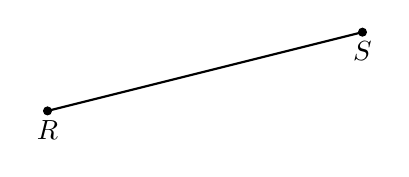
\begin{tikzpicture}
    \draw [-, thick] (0,0)--(4,1);
    \draw [fill] (0,0) circle [radius=0.05] node[below]{$R$};
    \draw [fill] (4,1) circle [radius=0.05] node[below]{$S$};
  \end{tikzpicture} \bigskip

\item Draw and label a line segment $AB$ such that the distance between points $A$ and $B$ is 8 cm. \vspace{2cm}

\item Find the value of $|2-7|$.

\item Identify three points in the given plane.\\[0.25in]
  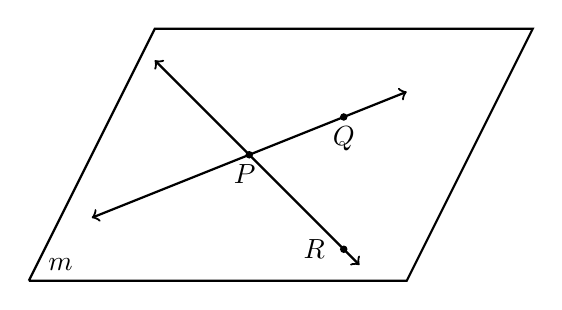
\begin{tikzpicture}[scale=0.8]
    \draw [thick](0,0) node[above right]{$\ m$} --(6,0)--(8,4)--(2,4)--(0,0);
    \draw [<->, thick] (1,1)--(6,3);
    \draw [fill] (3.5,2) circle [radius=0.05] node[below]{$P \ $};
    \draw [fill] (5,2.6) circle [radius=0.05] node[below]{$Q$};
    \draw [<->, thick] (2,3.5)--(5.25,.25);
    \draw [fill] (5,0.5) circle [radius=0.05] node[left]{$R \ $};
  \end{tikzpicture}

\item Given $M(2,3)$ and $N(5,9)$. What is the slope of $\overleftrightarrow{MN}$? Use the formula $\displaystyle m=\frac{y_2-y_1}{x_2-x_1}$. \vspace{3cm}

\item Given $\overline{DEF}$, $DE=10$, and $EF=3$. Find ${DF}$.\\[0.75cm]
    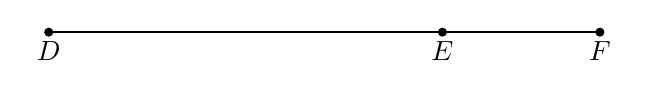
\begin{tikzpicture}
      \draw [-, thick] (0,0)--(7,0);
      \draw [fill] (0,0) circle [radius=0.05] node[below]{$D$};
      \draw [fill] (5,0) circle [radius=0.05] node[below]{$E$};
      \draw [fill] (7,0) circle [radius=0.05] node[below]{$F$};
    \end{tikzpicture} \smallskip

\newpage
\item Given $\triangle STU$ with $\overline{SU} \cong \overline{TU}$. On the diagram mark the congruent line segments with tick marks.
  \begin{center}
  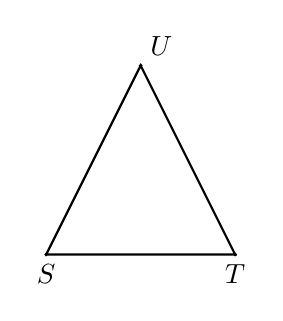
\begin{tikzpicture}[scale=0.3]
    \draw [thick](0,0)--(8,0)--(4,8)--(0,0);
    \draw [fill] (0,0) circle [radius=0.05] node[below]{$S$};
    \draw [fill] (8,0) circle [radius=0.05] node[below]{$T$};
    \draw [fill] (4,8) circle [radius=0.05] node[above right]{$U$};
  \end{tikzpicture}
  \end{center}

\item Given line segment $\overline{PQ}$ with midpoint $M$, that is, $\overline{PM} \cong \overline{QM}$. $PQ=14$ cm. Find the length of $\overline{MQ}$.\\[0.75cm]
  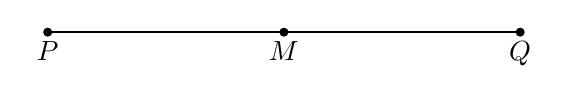
\begin{tikzpicture}
    \draw [-, thick] (0,0)--(6,0);
    \draw [fill] (0,0) circle [radius=0.05] node[below]{$P$};
    \draw [fill] (6,0) circle [radius=0.05] node[below]{$Q$};
    \draw [fill] (3,0) circle [radius=0.05] node[below]{$M$};
  \end{tikzpicture}
  \vspace{1cm}

\item Given the points $J$ and $K$, draw $\overrightarrow{JK}$.
  \begin{flushright}
    \begin{tikzpicture}
    \draw [fill] (0,2) circle [radius=0.05] node[below]{$K$};
    \draw [fill] (4,0) circle [radius=0.05] node[below]{$J$};
  \end{tikzpicture}
  \end{flushright}
  %\vspace{2cm}

\item Given $\overline{ABC}$, $AB=x+1$, $BC=3x-1$, and $AC=8$. Find ${AB}$.\\[0.5in]
      %\vspace{1cm}
     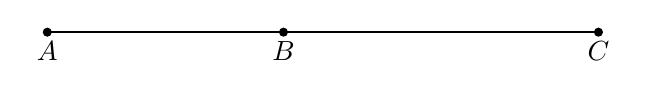
\begin{tikzpicture}
      \draw [-, thick] (0,0)--(7,0);
      \draw [fill] (0,0) circle [radius=0.05] node[below]{$A$};
      \draw [fill] (3,0) circle [radius=0.05] node[below]{$B$};
      \draw [fill] (7,0) circle [radius=0.05] node[below]{$C$};
    \end{tikzpicture} \vspace{2cm}

\newpage
\subsubsection*{Homework 1.6: Angle notation}
\item Write the appropriate name for the type of angle depending on its measure in degrees. (acute, right, obtuse, or straight)
  \begin{enumerate}
    \item $m\angle = 90$ : \rule{4cm}{0.15mm} \bigskip
    \item $90 < m\angle < 180$ : \rule{4cm}{0.15mm} \bigskip
    \item $0< m\angle < 90$ : \rule{4cm}{0.15mm} \bigskip
    \item $m\angle = 180$ : \rule{4cm}{0.15mm} \bigskip
  \end{enumerate}

\item Write down the name of the given angle three different ways.\\
  \begin{tikzpicture}
    \draw
      (3,-1) coordinate (a) node[right] {P}
      -- (0,0) coordinate (b) node[left] {Q}
      -- (2,2) coordinate (c) node[above right] {R}
      pic["1", <->, draw=black, angle eccentricity=1.2, angle radius=1cm]
      {angle=a--b--c};
  \end{tikzpicture}

\item Points that are all located on the same plane are $\rule{4cm}{0.15mm}$.

\item Write down the name of the angle shown in the diagram below using proper geometric notation.
  \begin{center}
  \begin{tikzpicture}[scale=2]
    \draw [->, thick] (0,0)--(4,3);
    \draw [->, thick] (0,0)--(5,-1);
    \draw [fill] (2.66666,2) circle [radius=0.05] node[above left ]{$D$};
    \draw [fill] (0,0) circle [radius=0.05] node[above left]{$E$};
    \draw [fill] (4,-0.8) circle [radius=0.05] node[above]{$F$};
  \end{tikzpicture}
  \end{center}
  Find the measure of the angle in degrees with a protractor.

\newpage
\item Given $\overline{ABC}$, $AB=3x-2$, $BC=x+11$, $AC=29$. Find ${AB}$. Show each step:\\[0.35in]
    \begin{flushright}
      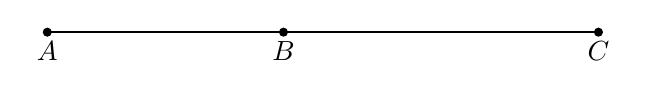
\begin{tikzpicture}
         \draw [-, thick] (0,0)--(7,0);
         \draw [fill] (0,0) circle [radius=0.05] node[below]{$A$};
         \draw [fill] (3,0) circle [radius=0.05] node[below]{$B$};
         \draw [fill] (7,0) circle [radius=0.05] node[below]{$C$};
      \end{tikzpicture}
    \end{flushright}
      %\vspace{1cm}
    \begin{enumerate}
      \item Sketch and label the situation
      \item Write a geometric equation:\\
      %\begin{flushright} Segment addition\\ postulate \end{flushright}
      \item Substitute algebraic values and solve:
      %\item Solve for the unknown
      \vspace{3cm}
      \begin{flushright} $x=$ \rule{1cm}{0.15mm} \end{flushright}
      \item Answer the question\\
      \begin{flushright} $AB=$ \rule{1cm}{0.15mm} \end{flushright}
      \item Check your answer
    \end{enumerate}

\item Given $\triangle ABC$ with $\overline{AC} \cong \overline{BC}$. $AC=5x+7$ and $BC=3x+17$. Find $AC$.\\[0.5cm]
    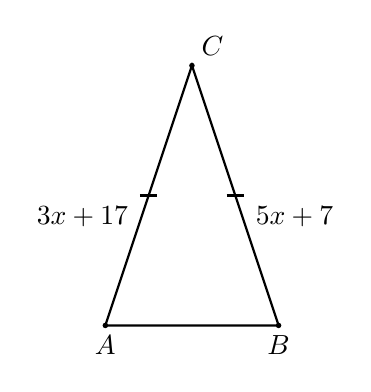
\begin{tikzpicture}[scale=0.55]
      \draw [thick](0,0)--(4,0)--(2,6)--(0,0);
      \draw [fill] (0,0) circle [radius=0.05] node[below]{$A$};
      \draw [fill] (4,0) circle [radius=0.05] node[below]{$B$};
      \draw [fill] (2,6) circle [radius=0.05] node[above right]{$C$};
      \draw [thick] (0.8,3)--(1.2,3); %tick mark
      \draw [thick] (2.8,3)--(3.2,3); %tick mark
      \node [right] at (3.25,2.5){$5x+7$};
      \node [left] at (0.75,2.5){$3x+17$};
    \end{tikzpicture}

\newpage
\subsubsection*{Quiz Corrections 1.6: Correct Friday's Do Now Quiz, complete this review, and staple them together. Due tomorrow for one-half of your missed points.} \bigskip
\item Segments of the same length, or angles having the same measure, are \ $\rule{3cm}{0.15mm}$.
  \bigskip

\item Use symbols to write the name of the given figure.
  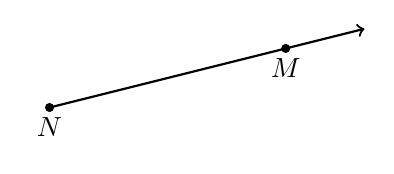
\begin{tikzpicture}
    \draw [->, thick] (0,0)--(4,1);
    \draw [fill] (0,0) circle [radius=0.05] node[below]{$N$};
    \draw [fill] (3,0.75) circle [radius=0.05] node[below]{$M$};
  \end{tikzpicture} \bigskip

\item Draw and label a line segment $AB$ such that the distance between points $A$ and $B$ is 6 cm. \vspace{2cm}

\item Find the value of $|11-4|+|-3|$.

\item Identify two rays in the given plane.\\[0.25in]
  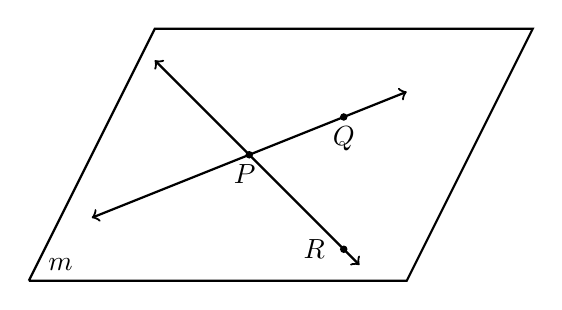
\begin{tikzpicture}[scale=0.8]
    \draw [thick](0,0) node[above right]{$\ m$} --(6,0)--(8,4)--(2,4)--(0,0);
    \draw [<->, thick] (1,1)--(6,3);
    \draw [fill] (3.5,2) circle [radius=0.05] node[below]{$P \ $};
    \draw [fill] (5,2.6) circle [radius=0.05] node[below]{$Q$};
    \draw [<->, thick] (2,3.5)--(5.25,.25);
    \draw [fill] (5,0.5) circle [radius=0.05] node[left]{$R \ $};
  \end{tikzpicture}

\item Given $T(7,4)$ and $U(5,8)$. What is the slope of $\overleftrightarrow{TU}$? Use the formula $\displaystyle m=\frac{y_U-y_T}{x_U-x_T}$. \vspace{3cm}

\item Given $\overline{DEF}$, $DE=4.5$, and $EF=1.5$. Find ${DF}$.\\[0.75cm]
    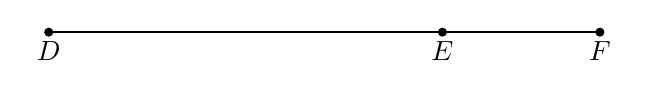
\begin{tikzpicture}
      \draw [-, thick] (0,0)--(7,0);
      \draw [fill] (0,0) circle [radius=0.05] node[below]{$D$};
      \draw [fill] (5,0) circle [radius=0.05] node[below]{$E$};
      \draw [fill] (7,0) circle [radius=0.05] node[below]{$F$};
    \end{tikzpicture} \smallskip

\newpage
\item Given $\triangle STU$ with $\overline{SU} \cong \overline{ST}$. On the diagram mark the congruent line segments with tick marks.
  \begin{center}
  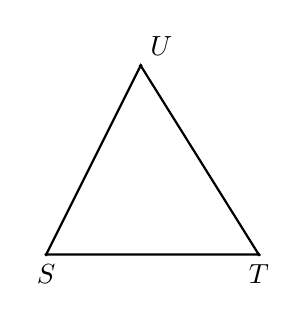
\begin{tikzpicture}[scale=0.3]
    \draw [thick](0,0)--(9,0)--(4,8)--(0,0);
    \draw [fill] (0,0) circle [radius=0.05] node[below]{$S$};
    \draw [fill] (9,0) circle [radius=0.05] node[below]{$T$};
    \draw [fill] (4,8) circle [radius=0.05] node[above right]{$U$};
  \end{tikzpicture}
  \end{center}

\item Given line segment $\overline{PQ}$ with midpoint $M$, that is, $\overline{PM} \cong \overline{QM}$. $PQ=20$ cm. Find the length of $\overline{MQ}$.\\[0.75cm]
  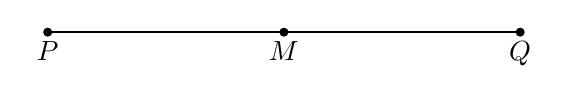
\begin{tikzpicture}
    \draw [-, thick] (0,0)--(6,0);
    \draw [fill] (0,0) circle [radius=0.05] node[below]{$P$};
    \draw [fill] (6,0) circle [radius=0.05] node[below]{$Q$};
    \draw [fill] (3,0) circle [radius=0.05] node[below]{$M$};
  \end{tikzpicture}
  \vspace{1cm}

\item Given the points $G$ and $H$, draw $\overleftrightarrow{GH}$.
  \begin{flushright}
    \begin{tikzpicture}
    \draw [fill] (0,2) circle [radius=0.05] node[below]{$G$};
    \draw [fill] (4,0) circle [radius=0.05] node[below]{$H$};
  \end{tikzpicture}
  \end{flushright}
  %\vspace{2cm}

\item Given $\overline{ABC}$, $AB=x+8$, $BC=2x-5$, and $AC=63$. Find ${AB}$.\\[0.5in]
      %\vspace{1cm}
     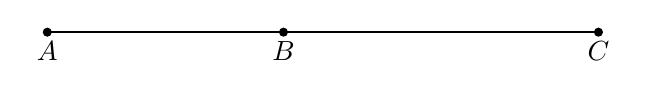
\begin{tikzpicture}
      \draw [-, thick] (0,0)--(7,0);
      \draw [fill] (0,0) circle [radius=0.05] node[below]{$A$};
      \draw [fill] (3,0) circle [radius=0.05] node[below]{$B$};
      \draw [fill] (7,0) circle [radius=0.05] node[below]{$C$};
    \end{tikzpicture} \vspace{2cm}

\newpage
\subsubsection*{Do Now 1.7: Angle measures}
\item For each example, explain the error made drawing $\overrightarrow{JK}$.\\.\\
  \vspace{0.5cm}
  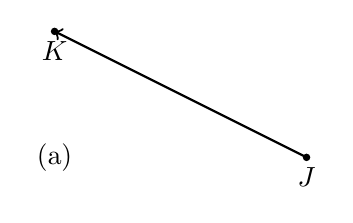
\begin{tikzpicture}[scale=.8]
    \draw  [<-, thick] (0,2)--(4,0);
    \draw [fill] (0,2) circle [radius=0.05] node[below]{$K$};
    \draw [fill] (4,0) circle [radius=0.05] node[below]{$J$};
    \node at (0,0) {(a)};
  \end{tikzpicture}  \hspace{1cm}
  \begin{tikzpicture}[scale=.8]
    \draw  [<-, thick] (-1,2.5)--(4.4,-0.2);
    \draw [fill] (0,2) circle [radius=0.05] node[below]{$K$};
    \draw [fill] (4,0) circle [radius=0.05] node[below left]{$J$};
    \node at (0,0) {(b)};
  \end{tikzpicture} \hspace{1cm}
  \begin{tikzpicture}[scale=.8]
    \draw  [<-, thick] (-1,2.5)--(0,2)--(2,1.1)--(3,0.4)--(4,0);
    \draw [fill] (0,2) circle [radius=0.05] node[below]{$K$};
    \draw [fill] (4,0) circle [radius=0.05] node[below]{$J$};
    \node at (0,0) {(c)};
  \end{tikzpicture}
  \vspace{2cm}

\item Write down the name of the \emph{three} angles shown in the diagram below and their angle measures, using your protractor. \vspace{1cm}
    \begin{center}
    \begin{tikzpicture}[scale=2]
      \draw [->, thick] (0,0)--(4,3);
      \draw [->, thick] (0,0)--(5,-.5);
      \draw [->, thick] (0,0)--(-1.2,3);
      \draw [fill] (-1,2.5) circle [radius=0.05] node[left ]{$B$};
      \draw [fill] (2.66666,2) circle [radius=0.05] node[above left ]{$C$};
      \draw [fill] (0,0) circle [radius=0.05] node[left]{$A$};
      \draw [fill] (4,-0.4) circle [radius=0.05] node[above]{$D$};
    \end{tikzpicture}
    \end{center}
    \begin{enumerate}
      \item  \rule{4cm}{0.15mm} \bigskip
      \item  \rule{4cm}{0.15mm} \bigskip
      \item  \rule{4cm}{0.15mm} \bigskip
    \end{enumerate}

\newpage
\item Given $\overline{ABC}$, $AB=5x-12$, $BC=x+4$, $AC=10$. Find ${BC}$.
    \begin{enumerate}
      \item Sketch and label the situation
      \begin{flushright}
        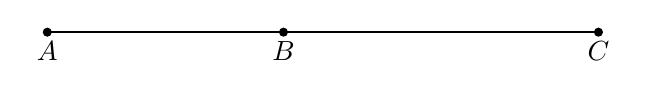
\begin{tikzpicture}
           \draw [-, thick] (0,0)--(7,0);
           \draw [fill] (0,0) circle [radius=0.05] node[below]{$A$};
           \draw [fill] (3,0) circle [radius=0.05] node[below]{$B$};
           \draw [fill] (7,0) circle [radius=0.05] node[below]{$C$};
        \end{tikzpicture}
      \end{flushright} \vspace{1cm}
      \item Write a geometric equation: \rule{5cm}{0.15mm} \vspace{1cm}
      \item Substitute algebraic values: \rule{5cm}{0.15mm}
      \item Solve for $x$
      \vspace{3cm}
      \begin{center} $x=$ \rule{1cm}{0.15mm} \end{center}
      \item Answer the question: Find $BC$ by substituting for $x$.\\
      \begin{center} $BC=($ \hspace{1cm} $)+4=$ \rule{1cm}{0.15mm} \end{center}
      \item Check your answer
    \end{enumerate}
    \vspace{2cm}

\item Given $\overrightarrow{DE}$, construct circle $E$ with radius $DE$.
    \vspace{3cm}
    \begin{center}
    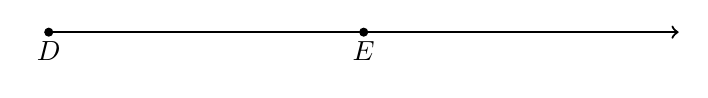
\begin{tikzpicture}
      \draw [->, thick] (0,0)--(8,0);
      \draw [fill] (0,0) circle [radius=0.05] node[below]{$D$};
      \draw [fill] (4,0) circle [radius=0.05] node[below]{$E$};
    \end{tikzpicture}
    \end{center}

\newpage
\subsubsection*{Homework 1.7: Angle addition postulate}
\item Given $m\angle LKM = 3x$, $m\angle MKN = x+20$, and $m\angle LKN = 100$, find $m\angle MKN$.  \vspace{1cm}
  \begin{enumerate}
    \item Sketch and label the situation
    \begin{flushright}
    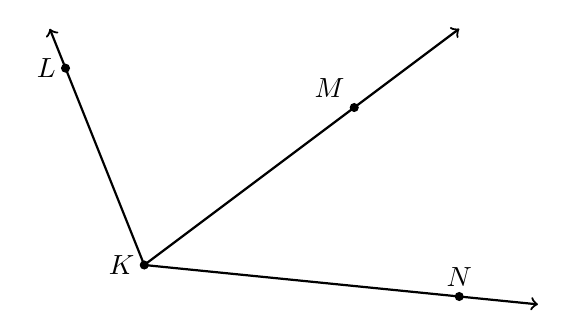
\begin{tikzpicture}[scale=1]
      \draw [->, thick] (0,0)--(4,3);
      \draw [->, thick] (0,0)--(5,-.5);
      \draw [->, thick] (0,0)--(-1.2,3);
      \draw [fill] (-1,2.5) circle [radius=0.05] node[left ]{$L$};
      \draw [fill] (2.66666,2) circle [radius=0.05] node[above left ]{$M$};
      \draw [fill] (0,0) circle [radius=0.05] node[left]{$K$};
      \draw [fill] (4,-0.4) circle [radius=0.05] node[above]{$N$};
    \end{tikzpicture}
    \end{flushright}
    \vspace{1cm}

  \item Write a geometric equation: \rule{5cm}{0.15mm} \vspace{1cm}
  \item Substitute algebraic values: \rule{5cm}{0.15mm}
  \item Solve for $x$
    \vspace{3cm}
    \begin{center} $x=$ \rule{1cm}{0.15mm} \end{center}
    \item Answer the question: Find $m\angle MKN$ by substituting for $x$.\\
    \begin{center} $m\angle MKN=($ \hspace{1cm} $)+20=$ \rule{1cm}{0.15mm} \end{center}
    \item Check your answer
  \end{enumerate}
  \vspace{2cm}

\newpage
\item Given $\overrightarrow{RS}$, construct circle $S$ with radius $RS$.\\
  Spicy: Complete the construction of an equilateral triangle with one side $\overline{RS}$.

  \vspace{4cm}
  \begin{center}
  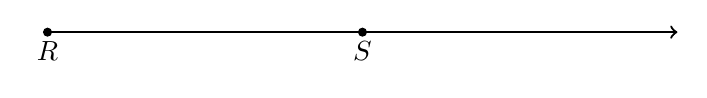
\begin{tikzpicture}
    \draw [->, thick] (0,0)--(8,0);
    \draw [fill] (0,0) circle [radius=0.05] node[below]{$R$};
    \draw [fill] (4,0) circle [radius=0.05] node[below]{$S$};
  \end{tikzpicture}
  \end{center}
  \vspace{4cm}

\item Given $\triangle ABC$ with $\overline{AC} \cong \overline{BC}$. $AC=4x-3$ and $BC=3x+7$. Find $AC$.\\[0.5cm]
  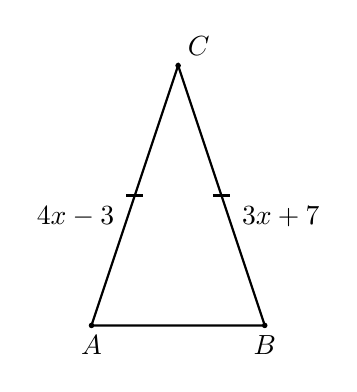
\begin{tikzpicture}[scale=0.55]
    \draw [thick](0,0)--(4,0)--(2,6)--(0,0);
    \draw [fill] (0,0) circle [radius=0.05] node[below]{$A$};
    \draw [fill] (4,0) circle [radius=0.05] node[below]{$B$};
    \draw [fill] (2,6) circle [radius=0.05] node[above right]{$C$};
    \draw [thick] (0.8,3)--(1.2,3); %tick mark
    \draw [thick] (2.8,3)--(3.2,3); %tick mark
    \node [right] at (3.25,2.5){$3x+7$};
    \node [left] at (0.75,2.5){$4x-3$};
  \end{tikzpicture}


\newpage
\subsubsection*{Do Now 1.8: Bisector and midpoint problems}
\item Use symbols to write the name of the given figure.
  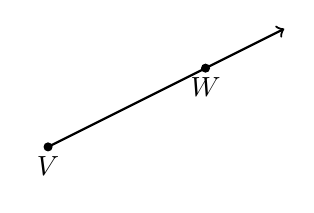
\begin{tikzpicture}
    \draw [->, thick] (0,0)--(3,1.5);
    \draw [fill] (0,0) circle [radius=0.05] node[below]{$V$};
    \draw [fill] (2,1) circle [radius=0.05] node[below]{$W$};
  \end{tikzpicture} \bigskip

\item A(n) $\rule{4cm}{0.15mm}$ is a portion of a line that begins with a single point and extends infinitely in one direction.

\item Given line segment $\overline{AB}$ with midpoint $M$, that is, $\overline{AM} \cong \overline{BM}$. $AM=5$ cm. Find $AB$.\\[0.75cm]
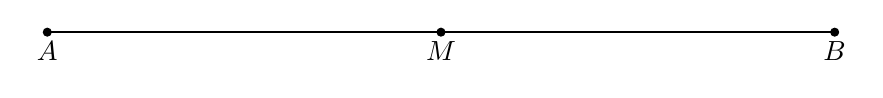
\begin{tikzpicture}
  \draw [-, thick] (0,0)--(10,0);
  \draw [fill] (0,0) circle [radius=0.05] node[below]{$A$};
  \draw [fill] (10,0) circle [radius=0.05] node[below]{$B$};
  \draw [fill] (5,0) circle [radius=0.05] node[below]{$M$};
\end{tikzpicture}
\vspace{1cm}

\item Given collinear points $P, Q, R$ with $Q$ bisecting the line segment $\overline{PR}$. $PQ=3x -12$ and $QR = x+6$. Find the length of $\overline{QR}$.\\First label the drawing.
  \begin{flushright}
  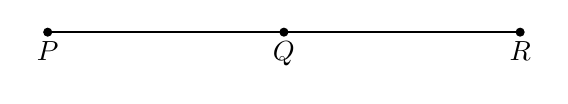
\begin{tikzpicture}
    \draw [-, thick] (0,0)--(6,0);
    \draw [fill] (0,0) circle [radius=0.05] node[below]{$P$};
    \draw [fill] (6,0) circle [radius=0.05] node[below]{$R$};
    \draw [fill] (3,0) circle [radius=0.05] node[below]{$Q$};
  \end{tikzpicture}
  \end{flushright}
  \begin{enumerate}
    \item Write a geometric equation: \rule{4cm}{0.15mm} \vspace{.7cm}
    \item Substitute algebraic values: \rule{4cm}{0.15mm}
    \item Solve for $x$
    \vspace{2.5cm}
    %\begin{center} $x=$ \rule{1cm}{0.15mm} \end{center}
    \item Answer the question: \bigskip
    \item Check your answer
  \end{enumerate}

\newpage
\item Given $\triangle ABC$ accurately measure the two sides in centimeters (cm) to the nearest tenth and $m \angle B$ in degrees.
    \bigskip
  \begin{enumerate}
    \item $AB= \rule{2cm}{0.15mm}$ \bigskip
    \item $BC= \rule{2cm}{0.15mm}$ \bigskip
    \item $m \angle ABC= \rule{2cm}{0.15mm}$
  \end{enumerate}
  \begin{center}
  \begin{tikzpicture} [scale=1.2]
    \draw [thick](0,0)--(8,1)--(2,4)--(0,0);
    \draw [fill] (0,0) circle [radius=0.05] node[below]{$A$};
    \draw [fill] (8,1) circle [radius=0.05] node[below]{$B$};
    \draw [fill] (2,4) circle [radius=0.05] node[above right]{$C$};
  \end{tikzpicture}
  \end{center}


\item Complete the construction of an equilateral triangle.
  \begin{enumerate}
    \item Construct circle $A$ with radius $AB$.
    \item Construct circle $B$ with radius $AB$.
    \item Label the intersection $C$ of the two circles.
    \item Draw line segments $\overline{AC}$ and $\overline{BC}$
  \end{enumerate}
  \vspace{4cm}
  \begin{center}
  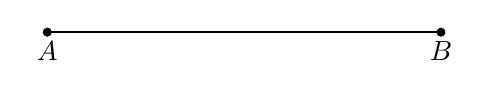
\begin{tikzpicture}
    \draw [-, thick] (0,0)--(5,0);
    \draw [fill] (0,0) circle [radius=0.05] node[below]{$A$};
    \draw [fill] (5,0) circle [radius=0.05] node[below]{$B$};
  \end{tikzpicture}
  \end{center}

\newpage
\subsubsection*{Do Now 1.8: Test review warmup problems}
\item Use symbols to write the name of the given figure.
    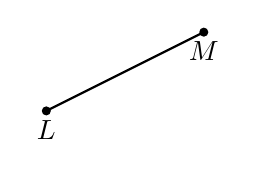
\begin{tikzpicture}
      \draw [-, thick] (0,0)--(2,1);
      \draw [fill] (0,0) circle [radius=0.05] node[below]{$L$};
      \draw [fill] (2,1) circle [radius=0.05] node[below]{$M$};
    \end{tikzpicture} \bigskip

\item Given $\triangle STU$ with $\overline{ST} \cong \overline{TU}$. On the diagram mark the congruent line segments with tick marks.
  \begin{center}
  \begin{tikzpicture}[scale=0.3]
    \draw [thick](0,0)--(9,0)--(4,8)--(0,0);
    \draw [fill] (0,0) circle [radius=0.05] node[below]{$S$};
    \draw [fill] (9,0) circle [radius=0.05] node[below]{$T$};
    \draw [fill] (4,8) circle [radius=0.05] node[above right]{$U$};
  \end{tikzpicture}
  \end{center}

\item Identify two line segments in the given plane.\\[0.25in]
    \begin{tikzpicture}[scale=0.8]
      \draw [thick](0,0) node[above right]{$\ m$} --(6,0)--(8,4)--(2,4)--(0,0);
      \draw [<->, thick] (1,1)--(6,3);
      \draw [fill] (3.5,2) circle [radius=0.05] node[below]{$P \ $};
      \draw [fill] (5,2.6) circle [radius=0.05] node[below]{$Q$};
      \draw [<->, thick] (2,3.5)--(5.25,.25);
      \draw [fill] (5,0.5) circle [radius=0.05] node[left]{$R \ $};
    \end{tikzpicture}

\item Find the measure of the angle in degrees and the given segment's length in centimeters. \vspace{0.25cm}
  \begin{enumerate}
    \item  $m \angle CAB = $ \rule{4cm}{0.15mm} \bigskip
    \item  $AB=$ \rule{4cm}{0.15mm} \bigskip
  \end{enumerate}
  \begin{center}
  \begin{tikzpicture}[scale=1.5]
    \draw [->, thick] (0,0)--(4,3);
    \draw [->, thick] (0,0)--(7,0);
    %\draw [->, thick] (0,0)--(-1.2,3);
    %\draw [fill] (-1,2.5) circle [radius=0.05] node[left ]{$B$};
    \draw [fill] (2.66666,2) circle [radius=0.05] node[above left ]{$C$};
    \draw [fill] (0,0) circle [radius=0.05] node[left]{$A$};
    \draw [fill] (4,0) circle [radius=0.05] node[above]{$B$};
  \end{tikzpicture}
  \end{center}

\newpage
\item Given line segment $\overline{XZ}$ with bisector $Y$. $YZ=4.2$ cm. Find $XY$.\\[1.5cm]
  \begin{tikzpicture}
    \draw [-, thick] (0,0)--(8,0);
    \draw [fill] (0,0) circle [radius=0.05] node[below]{$X$};
    \draw [fill] (8,0) circle [radius=0.05] node[below]{$Z$};
    \draw [fill] (4,0) circle [radius=0.05] node[below]{$Y$};
  \end{tikzpicture}
  \vspace{1cm}

\item Absolute value: Find the value of $|7-9|+|-3-1|$. \vspace{1cm}

\item Complete the construction of an equilateral triangle and fill in the blanks of the steps.
  \begin{enumerate}
    \item Given the line segment $\overline{GH}$. \bigskip
    \item Construct circle $G$ with radius $\rule{2cm}{0.15mm}$. \bigskip
    \item Construct circle $\rule{2cm}{0.15mm}$  with radius $\rule{2cm}{0.15mm}$. \bigskip
    \item Label the intersection $J$ of the two circles. \bigskip
    \item Draw line segments $\rule{2cm}{0.15mm}$  and $\rule{2cm}{0.15mm}$
    \item $\triangle GHJ$ is equilateral.
  \end{enumerate}
  \vspace{5cm}
  \begin{center}
  \begin{tikzpicture}
    \draw [-, thick] (0,0)--(6,0);
    \draw [fill] (0,0) circle [radius=0.05] node[below]{$G$};
    \draw [fill] (6,0) circle [radius=0.05] node[below]{$H$};
  \end{tikzpicture}
  \end{center}

\newpage
\subsubsection*{Homework 2.0: Weekend decompress}
\item Given $\triangle ABC$ with $\overline{AC} \cong \overline{BC}$. $AC=10x+1$ and $BC=8x+3$. Find $AC$.\\[0.5cm]
  \begin{tikzpicture}[scale=0.6]
    \draw [thick](0,0)--(4,0)--(2,6)--(0,0);
    \draw [fill] (0,0) circle [radius=0.05] node[below]{$A$};
    \draw [fill] (4,0) circle [radius=0.05] node[below]{$B$};
    \draw [fill] (2,6) circle [radius=0.05] node[above right]{$C$};
    \draw [thick] (0.8,3)--(1.2,3); %tick mark
    \draw [thick] (2.8,3)--(3.2,3); %tick mark
    \node [right] at (3.25,2.5){$8x+3$};
    \node [left] at (0.75,2.5){$10x+1$};
  \end{tikzpicture}
  \vspace{4cm}

\item Spicy: Given the rectangle $ABCD$ with $\overline{AB} \cong \overline{CD}$ and $\overline{BC} \cong \overline{DA}$. $AB=4x+\frac{3}{4}$ and $\displaystyle CD=\frac{7x+5}{2}$. Find $AB$.\\[0.5cm]
  \begin{tikzpicture}[scale=0.75]
    \draw [thick](0,0)--(6,0)--(6,3)--(0,3)--(0,0);
    \draw [fill] (0,0) circle [radius=0.05] node[below]{$A$};
    \draw [fill] (6,0) circle [radius=0.05] node[below]{$B$};
    \draw [fill] (6,3) circle [radius=0.05] node[above right]{$C$};
    \draw [fill] (0,3) circle [radius=0.05] node[above left]{$D$};
    \draw [thick] (3,-0.2)--(3,0.2); %tick mark
    \draw [thick] (3,2.8)--(3,3.2); %tick mark
    \draw [thick] (-0.2,1.4)--(0.2,1.4); %tick mark
    \draw [thick] (-0.2,1.6)--(0.2,1.6); %tick mark
    \draw [thick] (5.8,1.4)--(6.2,1.4); %tick mark
    \draw [thick] (5.8,1.6)--(6.2,1.6); %tick mark
    \node [below] at (2,0){$\displaystyle 4x+\frac{3}{4}$};
    \node [below] at (2,3){$\displaystyle \frac{7x+5}{2}$};
  \end{tikzpicture}
  %\vspace{4cm}

\end{enumerate}
\end{document}